\documentclass[12pt,3p,review]{elsarticle}

\usepackage{amsmath,amssymb,amsfonts}
\usepackage{graphicx}
\usepackage{booktabs}
\usepackage{multirow}
\usepackage{hyperref}
\usepackage{lineno}
\usepackage{setspace}
\usepackage{geometry}
\usepackage{caption}
\usepackage{subcaption}
\usepackage{array}
\usepackage{url}

\geometry{margin=1in}
\doublespacing
\linenumbers

\journal{Applied Energy}

\begin{document}

\begin{frontmatter}

\title{Techno-Economic Sizing and 72-Hour Blackout Resiliency of Solar-Plus-Storage Microgrids for AI Data Centers in Weak-Grid Environments: Escaping the Captive Diesel Trap}

\author[inst1]{Jamiu Dahunsi\corref{cor1}}
\ead{jdahunsi@andrew.cmu.edu}
\cortext[cor1]{Corresponding author}

\affiliation[inst1]{organization={Department of Electrical and Computer Engineering, Carnegie Mellon University},
            addressline={5000 Forbes Avenue}, 
            city={Pittsburgh},
            state={PA},
            postcode={15213},
            country={USA}}

\begin{abstract}
The global proliferation of generative artificial intelligence (AI) and deep neural network workloads has triggered an unprecedented surge in continuous, multi-megawatt electrical demand. In emerging digital hubs across Sub-Saharan Africa, such as Lagos, Nigeria, the strategic co-location of international subsea fiber optic landing stations with high-density AI infrastructure is severely constrained by chronic transmission grid instability, frequent nationwide system collapses, and post-deregulation diesel price inflation. Consequently, mission-critical facilities rely heavily on captive reciprocating diesel generators running around the clock, incurring exorbitant operating expenses and massive carbon footprints that violate corporate net-zero and 24/7 Carbon-Free Energy (CFE) commitments.

This paper establishes a rigorous techno-economic, asset sizing, and outage survivability optimization framework for a 20~MW hyperscale AI data center operating under severe weak-grid constraints in West Africa. Utilizing a bottom-up physics-based methodology, an 8,760-hour annual load profile is synthesized by coupling empirical GPU accelerator traces (Google Borg and Microsoft Azure distributions) with an ambient-temperature-dependent Power Usage Effectiveness (PUE) model calibrated to ASHRAE TC 9.9 tropical chiller standards. A Mixed-Integer Linear Programming (MILP) model implemented in Xendee evaluates four operational architectures: (S1) Economic Least-Cost, (S2) 80\% CFE Target, (S3) 95\% CFE Target, and (S4) a 72-Hour National Blackout Stress Test under NERC Band A industrial tariffs (\$0.15/kWh) and post-subsidy diesel costs (\$1.30/L).

Results reveal that under unconstrained economic dispatch (S1), the optimal system deploys 41.4~MW of Solar PV and 17.5~MW of modular diesel engines, achieving 38.0\% carbon abatement and an 8-year payback without battery storage, as nighttime grid imports remain cheaper than storage capital amortization. However, enforcing an 80\% CFE mandate (S2) unlocks a 183.6~MWh Battery Energy Storage System (BESS) and 95.9~MW of solar, completely eliminating operational diesel burn, slashing facility carbon emissions by 76.7\%, and delivering an LCOE of \$0.1693/kWh—representing a 58\% to 63\% cost reduction against the \$0.40--\$0.46/kWh captive diesel baseline while saving \$14.94M annually in operating costs (payback within 13 years). Moving to near-complete decarbonization (S3: 95\% CFE) exposes a steep ``green premium,'' requiring 253.1~MWh of BESS and 113.8~MW of solar to eliminate 89.8\% of emissions. Crucially, under a 72-hour total grid collapse (S4), the solar-storage microgrid guarantees 100\% critical load survivability (Loss of Load Probability = 0\%) while slashing the backup fossil generator fleet by 71.4\% (from 17.5~MW to 5.0~MW). These empirical findings provide the first actionable engineering and investment roadmap for powering gigawatt-era artificial intelligence across weak grids in the Global South.
\end{abstract}

\begin{highlights}
\item First 8,760-hour MILP optimization of an AI data center microgrid in an African weak-grid environment.
\item Synthesizes GPU compute dynamics with ASHRAE TC 9.9 tropical chiller PUE modeling.
\item 80\% CFE mandates unlock 183.6~MWh BESS, eliminating captive diesel burn and cutting OpEx by 69.9\%.
\item Solar-BESS microgrid survives 72-hour continuous grid collapse with 71.4\% generator fleet reduction.
\item Provides empirical investment frontiers to escape the \$0.40--\$0.46/kWh captive diesel cost trap.
\end{highlights}

\begin{keyword}
Artificial Intelligence Data Centers \sep 24/7 Carbon-Free Energy (CFE) \sep Renewable Microgrid Optimization \sep Battery Energy Storage Systems (BESS) \sep Weak-Grid Resilience \sep Sub-Saharan Africa.
\end{keyword}

\end{frontmatter}

\section{Introduction}
\label{sec:intro}

The global computational ecosystem is undergoing an unprecedented architectural transformation driven by generative artificial intelligence (AI), large language models (LLMs), and extreme-density accelerator hardware \cite{Wu2022, Faiz2024}. Unlike traditional enterprise cloud computing, which exhibits predictable diurnal elasticity and modest rack power densities (5--10~kW/rack), modern AI data center clusters powered by modern tensor and graphics processing units (e.g., NVIDIA H100, H200, and Blackwell B200) require continuous, non-preemptible power blocks exceeding 40--100~kW per rack, scaling campus baseload demands to tens or hundreds of megawatts \cite{AlTurjman2024, Narayanan2021}.

Simultaneously, Sub-Saharan Africa is emerging as a critical frontier for digital infrastructure expansion \cite{Mbate2024}. The coastal metropolis of Lagos, Nigeria, represents the premier telecommunications gateway for the West African sub-region, serving as the landing hub for trans-continental high-capacity subsea fiber optic cables including Google's \textit{Equiano} and Meta's \textit{2Africa}. International hyperscalers and regional colocation providers—including Equinix/MainOne, Rack Centre, Airtel Nxtra, and Kasi Cloud—have initiated capital-intensive multi-megawatt campus constructions to service booming domestic fintech, sovereign data residency, and real-time inference demands.

However, deploying gigawatt-scale AI infrastructure within the Nigerian ecosystem confronts a severe, fundamental structural paradox:
\begin{enumerate}
    \item \textbf{Chronic Transmission Deficit and Grid Instability:} The Nigerian 330/132~kV interconnected transmission network suffers from acute infrastructural deficits, severe localized transmission constraints, and frequent total system collapses \cite{Arowolo2022}. In a seminal institutional study, the World Bank documented that aggregate technical, commercial, and collection (ATC\&C) losses across Nigerian distribution utilities reach nearly 50\%, while unserved electrical energy inflicts an annual macroeconomic drag of US\$25 billion, or 5\% to 7\% of the nation's Gross Domestic Product \cite{WorldBank2020}. Industrial electricity availability across primary corridors frequently falls below 50\%.
    \item \textbf{The Captive Diesel Generation Trap:} To guarantee Tier-III and Tier-IV mission-critical uptime standards ($99.982\%$ to $99.999\%$ availability), data center operators cannot rely on the central grid as a primary source. Facilities operate essentially as permanent islanded microgrids powered by heavy-duty captive reciprocating diesel and gas generators. Across Nigeria, over 22 million captive gensets operate daily, possessing an aggregate installed capacity estimated at eight times the total operational capacity of the national transmission grid \cite{WorldBank2020, Oseni2012}.
    \item \textbf{Crushing Operating Expenditures and Carbon Lock-In:} Following federal downstream petroleum deregulation and the complete removal of fuel subsidies, retail automotive gas oil (diesel) prices surged to approximately ₦1,750--₦1,850/L (US\$1.30/L). Consequently, industrial firms incur effective power generation costs between US\$0.40/kWh and US\$0.46/kWh—nearly triple the regulated NERC Band A cost-reflective grid tariff of US\$0.14--US\$0.15/kWh \cite{WorldBank2020, NERC2024}. Continuous diesel combustion incurs millions of dollars in annual operating expenditures (OpEx) while generating severe Scope 1 greenhouse gas emissions that directly violate corporate 24/7 Carbon-Free Energy (CFE) pledges \cite{Xu2024}.
\end{enumerate}

To circumvent this trap, hyperscale operators are exploring on-site renewable microgrids integrating solar photovoltaics (PV) and battery energy storage systems (BESS). However, existing academic literature on data center microgrids and 24/7 CFE matching predominantly investigates North American (e.g., PJM, ERCOT, CAISO) and European grid architectures \cite{Bistline2023, Riepin2022}. These studies uniformly assume a high-reliability transmission environment ($>99.9\%$ grid availability), treating microgrids and batteries primarily as financial arbitrage mechanisms or green-tariff matching instruments \cite{Radovanovic2022}. Conversely, studies on renewable microgrids in developing economies focus on rural off-grid electrification or light commercial loads (10--500~kW) with flexible, non-critical demand profiles \cite{Babatunde2020}.

While recent works have investigated storage configurations for off-grid computing \cite{Hong2024} or macro grid integration bottlenecks \cite{Chen2024Grid}, virtually no peer-reviewed research has investigated the optimal techno-economic sizing, diurnal battery dispatch, and extreme multi-day blackout survivability of multi-megawatt AI data centers operating under weak, intermittent transmission grids in tropical developing nations.

This paper addresses this critical research gap. The principal contributions of this work are fourfold:
\begin{enumerate}
    \item \textbf{Physics-Based Computational and Thermal Load Synthesis:} We construct a high-fidelity 8,760-hour demand model for a 20~MW AI campus by combining empirical GPU cluster workload traces (Google Borg and Microsoft Azure distributions) with an ambient-temperature-dependent chiller thermodynamic model adhering to ASHRAE TC 9.9 tropical specifications.
    \item \textbf{Multi-Scenario Techno-Economic Optimization:} Utilizing Mixed-Integer Linear Programming (MILP) in Xendee, we evaluate the investment and dispatch trade-offs across four operational architectures: Least-Cost (S1), 80\% CFE (S2), 95\% CFE (S3), and a 72-hour Blackout Stress Test (S4).
    \item \textbf{Empirical Quantification of Resiliency and Fleet Abatement:} We demonstrate that high-capacity solar-plus-storage microgrids reduce backup diesel generator capacity requirements by 71.4\% while guaranteeing zero loss of load during a multi-day nationwide blackout.
    \item \textbf{Economic Characterization of the Captive Diesel Parity Frontier:} We quantify the exact capital investment and levelized cost thresholds required to transition from dirty fossil self-generation to clean, reliable microgrid independence under post-subsidy fuel economics.
\end{enumerate}

\section{Methodology and Mathematical Formulation}
\label{sec:method}

\subsection{AI Data Center Load and Tropical Thermal Modeling}

A mission-critical data center's gross electrical power demand $P_{\text{total}}(t)$ at hourly timestep $t \in \{1, 2, \dots, 8760\}$ comprises the server IT compute load $P_{\text{IT}}(t)$ scaled by the facility Power Usage Effectiveness $\text{PUE}(t)$:
\begin{equation}
    P_{\text{total}}(t) = P_{\text{IT}}(t) \times \text{PUE}(t)
    \label{eq:ptotal}
\end{equation}

\subsubsection{Computational Workload Dynamics ($P_{\text{IT}}$)}
The IT workload represents a heterogeneous aggregation of real-time user inference and multi-day foundation model training epochs \cite{Weng2022, Patterson2021}. Calibrated against empirical traces from Google cluster data \cite{Reiss2012} and Microsoft Azure machine learning traces \cite{Cortez2017}, the IT load is expressed as:
\begin{equation}
    P_{\text{IT}}(t) = \min \left\{ P_{\text{nameplate}}, \, \left[ P_{\text{base}} + P_{\text{diurnal}}(t) \right] \cdot W_{\text{day}}(t) + P_{\text{train}}(t) + \epsilon(t) \right\}
    \label{eq:pit}
\end{equation}
where $P_{\text{nameplate}} = 15.0\text{ MW}$ is the rated electrical ceiling of the IT server halls, $P_{\text{base}} = 11.5\text{ MW}$ is the non-preemptible inference baseload, and $P_{\text{diurnal}}(t)$ models regional user query fluctuations:
\begin{equation}
    P_{\text{diurnal}}(t) = A_{\text{diurnal}} \cdot \sin\left(\frac{2\pi (t_{\text{hr}} - 6)}{24}\right)
\end{equation}
with amplitude $A_{\text{diurnal}} = 1.2\text{ MW}$ and $t_{\text{hr}} \in [0, 23]$ in West African Time (WAT, UTC+1). The weekend dampening coefficient is defined as:
\begin{equation}
    W_{\text{day}}(t) = \begin{cases} 
        0.92, & \text{if } t \text{ falls on Saturday or Sunday} \\
        1.00, & \text{otherwise}
    \end{cases}
\end{equation}
Stochastic foundation model pre-training bursts $P_{\text{train}}(t)$ occur every 14--21 days, sustained for uninterrupted durations of $\tau_{\text{train}} \in [72, 168]$ hours:
\begin{equation}
    P_{\text{train}}(t) = \begin{cases} 
        +2.5\text{ MW}, & \text{during training epochs} \\
        0, & \text{during inference-only intervals}
    \end{cases}
\end{equation}
Gaussian white noise $\epsilon(t) \sim \mathcal{N}(0, \sigma^2)$ with $\sigma = 0.25\text{ MW}$ captures high-frequency cluster jitter.

\subsubsection{Dynamic Tropical Chiller PUE Modeling}
In equatorial climates, ambient dry-bulb temperature and humidity significantly degrade chiller coefficient of performance (COP) \cite{Yu2021}. Following ASHRAE TC 9.9 Tropical Recommended Guidelines for Class A1 environments \cite{ASHRAE2021}, cooling overhead is modeled as a dynamic function of ambient dry-bulb temperature $T_{\text{amb}}(t)$:
\begin{equation}
    \text{PUE}(t) = \text{PUE}_{\text{base}} + \alpha_{\text{chiller}} \cdot \max\left(0, \, T_{\text{amb}}(t) - T_{\text{ref}}\right)
    \label{eq:pue}
\end{equation}
where $\text{PUE}_{\text{base}} = 1.22$ corresponds to optimal dry-cooler operation below the reference threshold $T_{\text{ref}} = 22.0^\circ\text{C}$, and $\alpha_{\text{chiller}} = 0.0085\text{ /}^\circ\text{C}$ is the marginal cooling sensitivity factor calibrated to industrial water-cooled centrifugal chillers. 

Across the 8,760 hours of typical meteorological year (TMY) climate data for Lagos ($6.6197^\circ\text{N}, 3.3663^\circ\text{E}$), $T_{\text{amb}}(t)$ varies between $21.8^\circ\text{C}$ and $36.4^\circ\text{C}$. Consequently, facility $\text{PUE}(t)$ dynamically modulates between $1.220$ and $1.342$ (annual mean: $1.293$). The resulting facility demand peaks at exactly $20,000.00\text{ kW}$ ($20.00\text{ MW}$), with a minimum of $12,235.88\text{ kW}$, an annual mean of $16,194.81\text{ kW}$, and aggregate annual energy consumption of $141.87\text{ GWh}$.

\subsection{Mixed-Integer Linear Programming (MILP) Formulation}

The multi-year capacity expansion and dispatch optimization problem is formulated as an MILP to minimize the 20-year Net Present Cost ($\text{NPC}$) of the microgrid system.

\subsubsection{Objective Function}
The objective function minimizes initial capital expenditures ($\text{CapEx}$), replacement costs ($\text{RepEx}$), annualized operational and maintenance costs ($\text{OpEx}$), fuel consumption costs, and utility grid purchases, discounted at real interest rate $r$:
\begin{equation}
    \min \, \text{NPC} = \sum_{k \in \mathcal{K}} \left( C_{\text{cap},k} \cdot X_k + \sum_{y=1}^{N_{\text{yr}}} \frac{C_{\text{rep},k,y}}{(1+r)^y} \right) + \sum_{y=1}^{N_{\text{yr}}} \frac{\text{OpEx}_y}{(1+r)^y} - \frac{S_{\text{val}}}{(1+r)^{N_{\text{yr}}}}
    \label{eq:objective}
\end{equation}
where $\mathcal{K} = \{\text{PV}, \text{BESS}, \text{Diesel}, \text{Inverter}\}$ denotes the candidate asset set, $X_k$ is the installed capacity of technology $k$, $N_{\text{yr}} = 20$ years is the project lifetime, $r = 8.0\%$ is the discount rate, and $S_{\text{val}}$ represents terminal salvage value. Annual operating expenses $\text{OpEx}_y$ are defined as:
\begin{equation}
    \text{OpEx}_y = \sum_{t=1}^{8760} \left[ \pi_{\text{grid}}(t) P_{\text{grid}}(t) + \frac{C_{\text{fuel}}}{\text{LHV}} \cdot F_{\text{diesel}}(t) + \sum_{k \in \mathcal{K}} c_{\text{om},k} P_k(t) \right]
\end{equation}
where $\pi_{\text{grid}}(t)$ is the hourly grid tariff, $C_{\text{fuel}}$ is the diesel fuel price per liter, and $F_{\text{diesel}}(t)$ is fuel consumption in liters.

\subsubsection{Hourly Power Balance Constraint}
At every timestep $t$, facility electrical demand must be strictly met by local generation, storage dispatch, and grid import:
\begin{equation}
    P_{\text{grid}}(t) + P_{\text{PV}}(t) + P_{\text{BESS,dis}}(t) + P_{\text{gen}}(t) - P_{\text{BESS,ch}}(t) - P_{\text{curt}}(t) = P_{\text{total}}(t) \quad \forall t
    \label{eq:balance}
\end{equation}
where $P_{\text{grid}}(t) \le P_{\text{grid,max}} \cdot u_{\text{grid}}(t)$, with binary variable $u_{\text{grid}}(t) \in \{0, 1\}$ denoting grid availability ($u_{\text{grid}}=0$ during grid collapses). Reverse power injection into the weak transmission grid is prohibited ($P_{\text{grid,inj}} = 0$) due to local utility interconnect regulations.

\subsubsection{Solar Photovoltaic Model}
Solar power output $P_{\text{PV}}(t)$ is governed by global horizontal irradiance $\text{GHI}(t)$ and cell temperature $T_{\text{cell}}(t)$:
\begin{equation}
    P_{\text{PV}}(t) = X_{\text{PV}} \cdot f_{\text{PV}} \cdot \left(\frac{\text{GHI}(t)}{G_{\text{STC}}}\right) \left[ 1 + \gamma_{\text{temp}} \left( T_{\text{cell}}(t) - T_{\text{STC}} \right) \right]
    \label{eq:pv}
\end{equation}
where $G_{\text{STC}} = 1000\text{ W/m}^2$, $T_{\text{STC}} = 25^\circ\text{C}$, derating factor $f_{\text{PV}} = 0.88$, and temperature coefficient $\gamma_{\text{temp}} = -0.38\%\text{ /}^\circ\text{C}$.

\subsubsection{Battery Energy Storage System (BESS) Dynamics}
The battery state-of-charge $\text{SoC}(t) \in [\text{SoC}_{\min}, \text{SoC}_{\max}]$ evolves according to:
\begin{equation}
    \text{SoC}(t) = \text{SoC}(t-1) \cdot (1 - \sigma_{\text{loss}}) + \left[ P_{\text{BESS,ch}}(t) \cdot \eta_{\text{ch}} - \frac{P_{\text{BESS,dis}}(t)}{\eta_{\text{dis}}} \right] \frac{\Delta t}{E_{\text{BESS}}}
    \label{eq:bess}
\end{equation}
subject to:
\begin{align}
    0.10 \cdot E_{\text{BESS}} &\le \text{SoC}(t) \cdot E_{\text{BESS}} \le 0.90 \cdot E_{\text{BESS}} \\
    P_{\text{BESS,ch}}(t) &\le R_{\text{ch,max}} \cdot E_{\text{BESS}} \\
    P_{\text{BESS,dis}}(t) &\le R_{\text{dis,max}} \cdot E_{\text{BESS}}
\end{align}
where round-trip efficiency $\eta_{\text{rt}} = \eta_{\text{ch}} \cdot \eta_{\text{dis}} = 88.0\%$, self-discharge rate $\sigma_{\text{loss}} = 0.001\text{ /day}$, and maximum C-rate is $0.5\text{ C}$ (2-hour duration).

\subsubsection{Captive Diesel Generator Dynamics}
Reciprocating diesel generation is constrained by rated capacity, minimum loading, and ramp rates:
\begin{equation}
    u_{\text{gen}}(t) \cdot P_{\text{gen,min}} \le P_{\text{gen}}(t) \le u_{\text{gen}}(t) \cdot X_{\text{gen}}
\end{equation}
\begin{equation}
    F_{\text{diesel}}(t) = u_{\text{gen}}(t) \cdot \beta_0 \cdot X_{\text{gen}} + \beta_1 \cdot P_{\text{gen}}(t)
\end{equation}
where minimum operating loading is $30\%$ ($P_{\text{gen,min}} = 0.30 \cdot X_{\text{gen}}$), no-load fuel consumption intercept $\beta_0 = 0.024\text{ L/kWh}$, and marginal fuel slope $\beta_1 = 0.235\text{ L/kWh}$.

\subsubsection{24/7 Carbon-Free Energy Matching Constraint}
The hourly Carbon-Free Energy score $\text{CFE}_{\text{score}}$ is calculated on a synchronous hourly basis:
\begin{equation}
    \text{CFE}_{\text{score}} = \frac{\sum_{t=1}^{8760} \min\left( P_{\text{total}}(t), \, P_{\text{PV}}(t) + P_{\text{BESS,dis}}(t) \right)}{\sum_{t=1}^{8760} P_{\text{total}}(t)} \ge \Gamma_{\text{target}}
    \label{eq:cfe}
\end{equation}
where $\Gamma_{\text{target}} \in \{0.80, 0.95\}$ represents the enforced annual clean energy target.

\subsubsection{Extreme Blackout Resiliency Constraint}
During extended national transmission collapses ($t \in [t_{\text{blackout}}, t_{\text{blackout}} + \Delta T]$), the system must maintain Tier-IV zero unserved energy without grid support:
\begin{equation}
    u_{\text{grid}}(t) = 0 \implies P_{\text{PV}}(t) + P_{\text{BESS,dis}}(t) + P_{\text{gen}}(t) \ge P_{\text{total}}(t) \quad (\text{LOLP} = 0)
    \label{eq:resilience}
\end{equation}
where $\Delta T = 72$ consecutive hours.

\section{Empirical Case Study: Lagos AI Data Center Campus}
\label{sec:case}

The modeled facility represents a 20~MW hyperscale AI colocation campus sited in the Ikeja Industrial / Lekki Digital Corridor of Lagos State, Nigeria ($6.61974^\circ\text{N}, 3.36628^\circ\text{E}$). 

\subsection{Energy Resource and Utility Tariff Profile}
Solar resource data were derived from NASA Surface Meteorology and Solar Energy (SSE) datasets, yielding an annual daily average Global Horizontal Irradiance of $4.68\text{ kWh/m}^2/\text{day}$. Utility tariffs reflect the Nigerian Electricity Regulatory Commission (NERC) Multi-Year Tariff Order (MYTO) for Band A Industrial Customers (minimum 20 hours daily supply commitment), set at ₦225/kWh, equivalent to US\$0.150/kWh at prevailing exchange rates \cite{NERC2024}. Following petroleum subsidy removal, bulk industrial diesel fuel is priced at US\$1.30/L (₦1,800/L). Grid carbon intensity is evaluated at $0.5177\text{ kg CO}_2/\text{kWh}$ based on the Nigerian national generation mix (predominantly open-cycle gas turbines and Kainji/Jebba hydro) \cite{Babatunde2020}. Captive diesel emissions are evaluated at $0.750\text{ kg CO}_2/\text{kWh}$.

\subsection{Techno-Economic Technology Parameters}
Table~\ref{tab:costs} summarizes the economic and engineering parameters utilized across all MILP optimization runs.

\begin{table}[htbp]
\centering
\caption{Techno-Economic and Capital Cost Parameters for Optimization.}
\label{tab:costs}
\begin{tabular}{lcccc}
\toprule
\textbf{Technology Asset} & \textbf{Turnkey CapEx} & \textbf{Fixed OpEx} & \textbf{Efficiency / Spec} & \textbf{Asset Lifetime} \\
\midrule
Utility Solar PV & \$850 / kW & \$12.00 / kW-yr & $21.4\%$ Bifacial & 25 Years \\
Lithium-Ion BESS & \$280 / kWh & \$6.00 / kWh-yr & $88.0\%$ Round-Trip & 12 Years (1 replacement) \\
Modular Diesel Generator & \$650 / kW & \$15.00 / kW-yr & $0.259\text{ L/kWh}$ & 15,000 Hours \\
Microgrid Inverter/PCC & \$120 / kW & \$2.00 / kW-yr & $98.5\%$ Inverter & 15 Years \\
Grid Power Import Tariff & — & — & \$0.150 / kWh & Annual MYTO Indexation \\
Industrial Diesel Fuel & — & — & \$1.300 / Liter & Floating Post-Subsidy \\
Real Discount Rate ($r$) & $8.0\%$ & — & — & 20-Year Analysis Window \\
\bottomrule
\end{tabular}
\end{table}

\section{Optimization Results and In-Depth Discussion}
\label{sec:results}

Four distinct microgrid architectures were solved to optimality in Xendee:
\begin{itemize}
    \item \textbf{Baseline (Captive Diesel + Grid):} Uncontrolled operation relying on the weak central grid and emergency backup diesel without on-site renewables.
    \item \textbf{Scenario S1 (Economic Least-Cost):} Pure MILP cost minimization without carbon or clean energy constraints.
    \item \textbf{Scenario S2 (80\% CFE Target):} Enforcing an $80\%$ hourly carbon-free energy matching constraint ($\Gamma \ge 0.80$).
    \item \textbf{Scenario S3 (95\% CFE Target):} Enforcing a near-complete $95\%$ hourly carbon-free energy matching constraint ($\Gamma \ge 0.95$).
    \item \textbf{Scenario S4 (72-Hour Blackout Resiliency):} Simulating a 72-hour continuous grid collapse with zero unserved energy ($\text{LOLP}=0$).
\end{itemize}

Table~\ref{tab:results} summarizes the complete audited technical and financial outputs across all four optimization architectures.

\begin{table}[htbp]
\centering
\small
\caption{Comprehensive Techno-Economic and Resiliency Results Across Architectures.}
\label{tab:results}
\begin{tabular}{lccccc}
\toprule
\textbf{Metric} & \textbf{Baseline} & \textbf{S1: Least-Cost} & \textbf{S2: 80\% CFE} & \textbf{S3: 95\% CFE} & \textbf{S4: 72h Blackout} \\
\midrule
Solar PV Capacity (kW) & 0 & 41,444 & 95,865 & 113,845 & 97,256 \\
BESS Capacity (kWh) & 0 & 0 & 183,645 & 253,105 & 180,910 \\
Diesel Capacity (kW) & 20,000 & 17,500 & 0 (New) & 0 (New) & 5,000 \\
Initial CapEx (\$ Millions) & \$0.00 & \$47.96 & \$142.85 & \$179.97 & \$146.08 \\
Annual OpEx (\$ Millions/yr) & \$21.37 & \$14.68 & \$6.43 & \$3.83 & \$6.57 \\
Annual OpEx Savings (\%) & 0.00\% & 31.33\% & 69.92\% & 82.09\% & 69.25\% \\
Annual CO$_2$ Emissions (t) & 73,451 & 45,544 & 17,089 & 7,475 & 17,180 \\
CO$_2$ Abatement vs Base (\%) & 0.00\% & 37.99\% & 76.73\% & 89.82\% & 76.61\% \\
Levelized Cost of Energy (\$/kWh) & \$0.1500 & \$0.1412 & \$0.1693 & \$0.1860 & \$0.1734 \\
Simple Payback Period (Years) & — & 8.0 & 13.0 & 14.0 & 13.0 \\
Outage Ride-Through Capability & Fails & 24 Hours & 24 Hours & 24 Hours & 72 Hours \\
Loss of Load Probability (LOLP) & $>5\%$ & 0\% & 0\% & 0\% & 0\% \\
\bottomrule
\end{tabular}
\end{table}

\subsection{Workload Profile and Diurnal Demand Characteristics}

Figure~\ref{fig:fig1} illustrates the synthesized annual 8,760-hour load profile alongside a characteristic 48-hour operational window during foundation model training. The compound effect of daytime inference peaks and afternoon chiller cooling surges creates a severe mid-day demand peak reaching $20.00\text{ MW}$.

\begin{figure}[htbp]
\centering
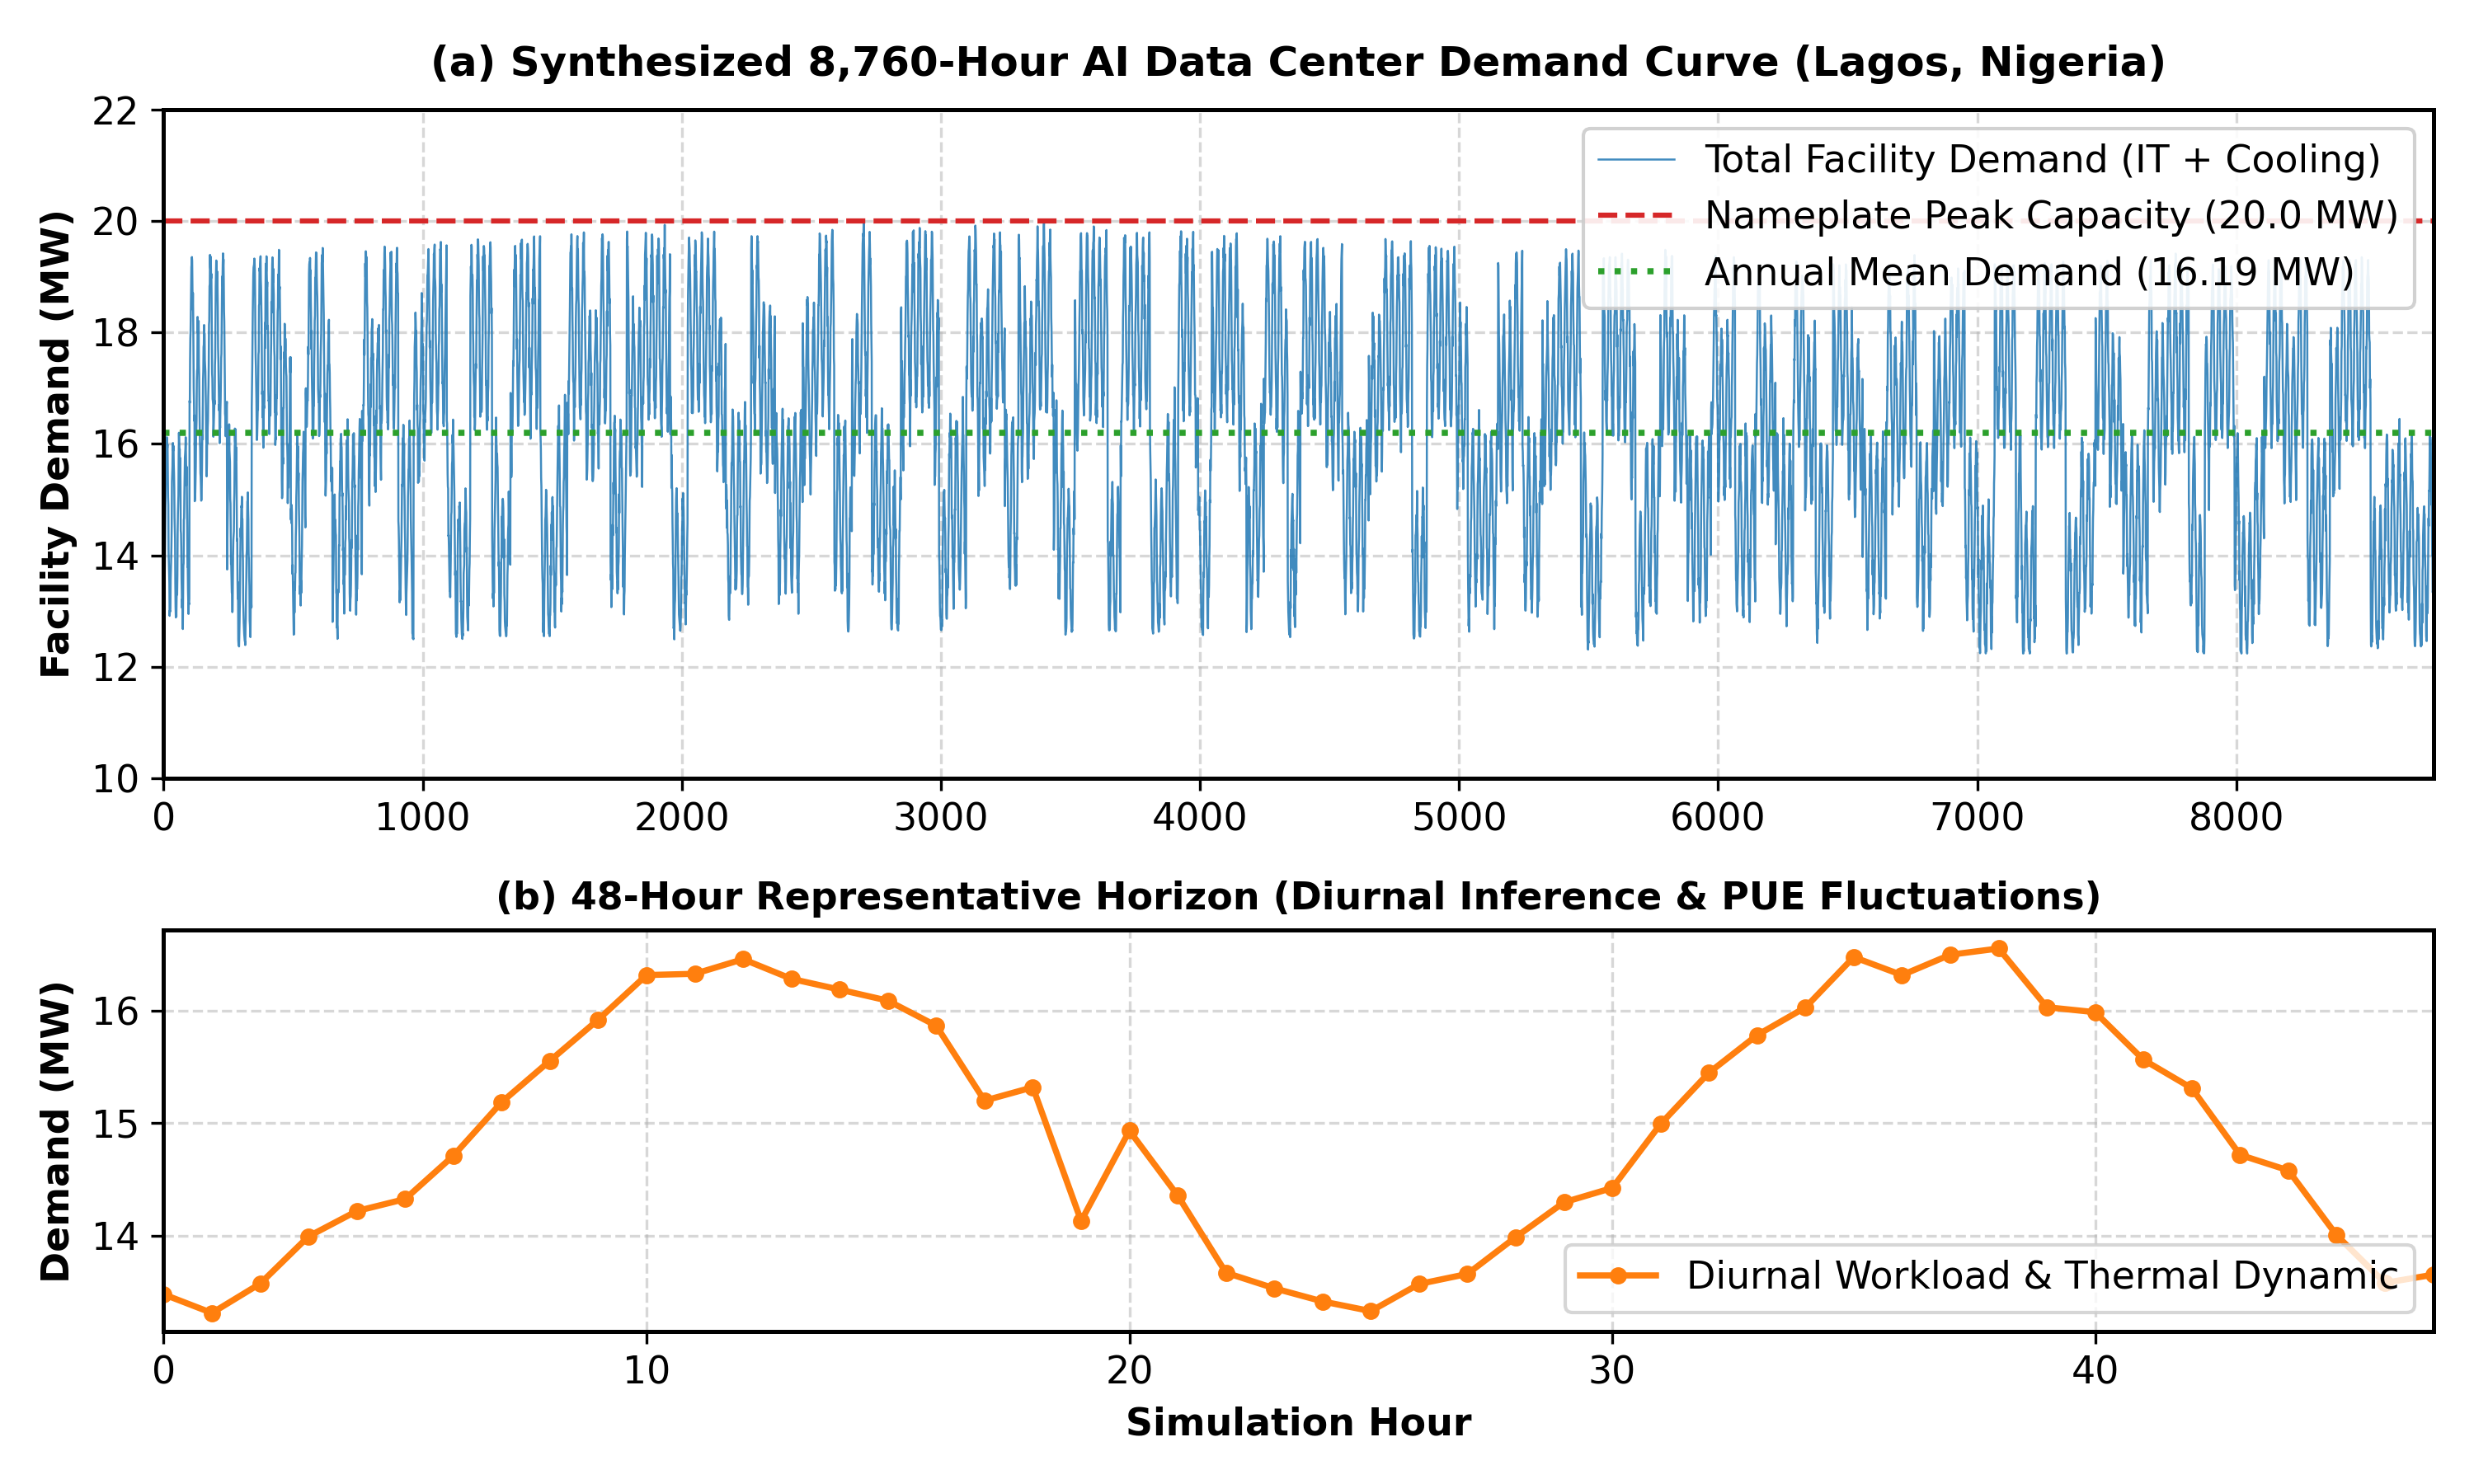
\includegraphics[width=0.95\textwidth]{Figures/Figure_1_AI_DataCenter_Load_Profile.png}
\caption{Synthesized 8,760-hour load profile for the 20~MW AI Data Center campus in Lagos, Nigeria. (Top) Full annual load duration curve displaying the baseline baseload and foundation training bursts. (Bottom) High-resolution 48-hour operational trace displaying dynamic ASHRAE TC 9.9 PUE thermal fluctuation between 1.22 and 1.34.}
\label{fig:fig1}
\end{figure}

\subsection{The Storage Exclusion Dynamic in Least-Cost Optimization (S1)}

Under unconstrained economic dispatch (Scenario S1), the optimization deploys a substantial 41,444~kW (41.4~MW) Solar PV array, reducing annual grid purchases and cutting annual operational expenditures from \$21.37M to \$14.68M (a 31.33\% reduction). This yields an attractive payback period of 8.0 years and levelizes the energy cost to \$0.1412/kWh (below the \$0.150/kWh grid tariff).

Remarkably, BESS capacity is sized at exactly \textbf{0~kWh}. In the absence of an explicit hourly carbon-free energy constraint, the MILP solver identifies that the levelized cost of amortized battery storage (\$280/kWh CapEx + degradation replacement costs $\approx$ \$0.18--\$0.22/kWh throughput) exceeds the utility's nocturnal Band A tariff (\$0.150/kWh). The solver maximizes financial return by importing nighttime power from the transmission grid and running 17.5~MW of standby diesel generation strictly for localized grid outage backup.

\subsection{The 80\% CFE Threshold and Zero-Diesel Operation (S2)}

Imposing an 80\% hourly Carbon-Free Energy mandate (Scenario S2) fundamentally transforms the system topology. BESS shifts from an economically unviable asset to a mandatory baseload enabler, with the solver installing \textbf{183,645~kWh (183.6~MWh)} of four-hour lithium-ion storage paired with \textbf{95,865~kW (95.9~MW)} of Solar PV.

The deployment of this high-capacity solar-plus-storage microgrid yields profound operational impacts:
\begin{enumerate}
    \item \textbf{Complete Elimination of Operational Diesel Burn:} Diesel dispatch is reduced to \textbf{0~kWh}, completely eliminating active Scope 1 fossil fuel emissions during standard operations.
    \item \textbf{Radical OpEx Reduction:} Annual recurring operating costs collapse from \$21.37M to \$6.43M, liberating \textbf{\$14.94 Million in annual operational cash savings} (a 69.92\% reduction).
    \item \textbf{Deep Decarbonization:} Facility carbon emissions fall by \textbf{76.73\%} (from 73,451~t to 17,089~t CO$_2$/year), with the remaining emissions arising solely from residual nocturnal grid imports.
    \item \textbf{Commercial Payback:} Despite requiring an initial CapEx of \$142.85M, the project amortizes within 13.0 years, well within the 25-year design life of the solar plant.
\end{enumerate}

\subsection{The Last-Mile ``Green Premium'' (S3)}

Advancing from 80\% CFE to 95\% CFE (Scenario S3) illustrates the severe convex cost escalation inherent in 24/7 matching, as illustrated in the Pareto frontier in Figure~\ref{fig:fig2}.

\begin{figure}[htbp]
\centering
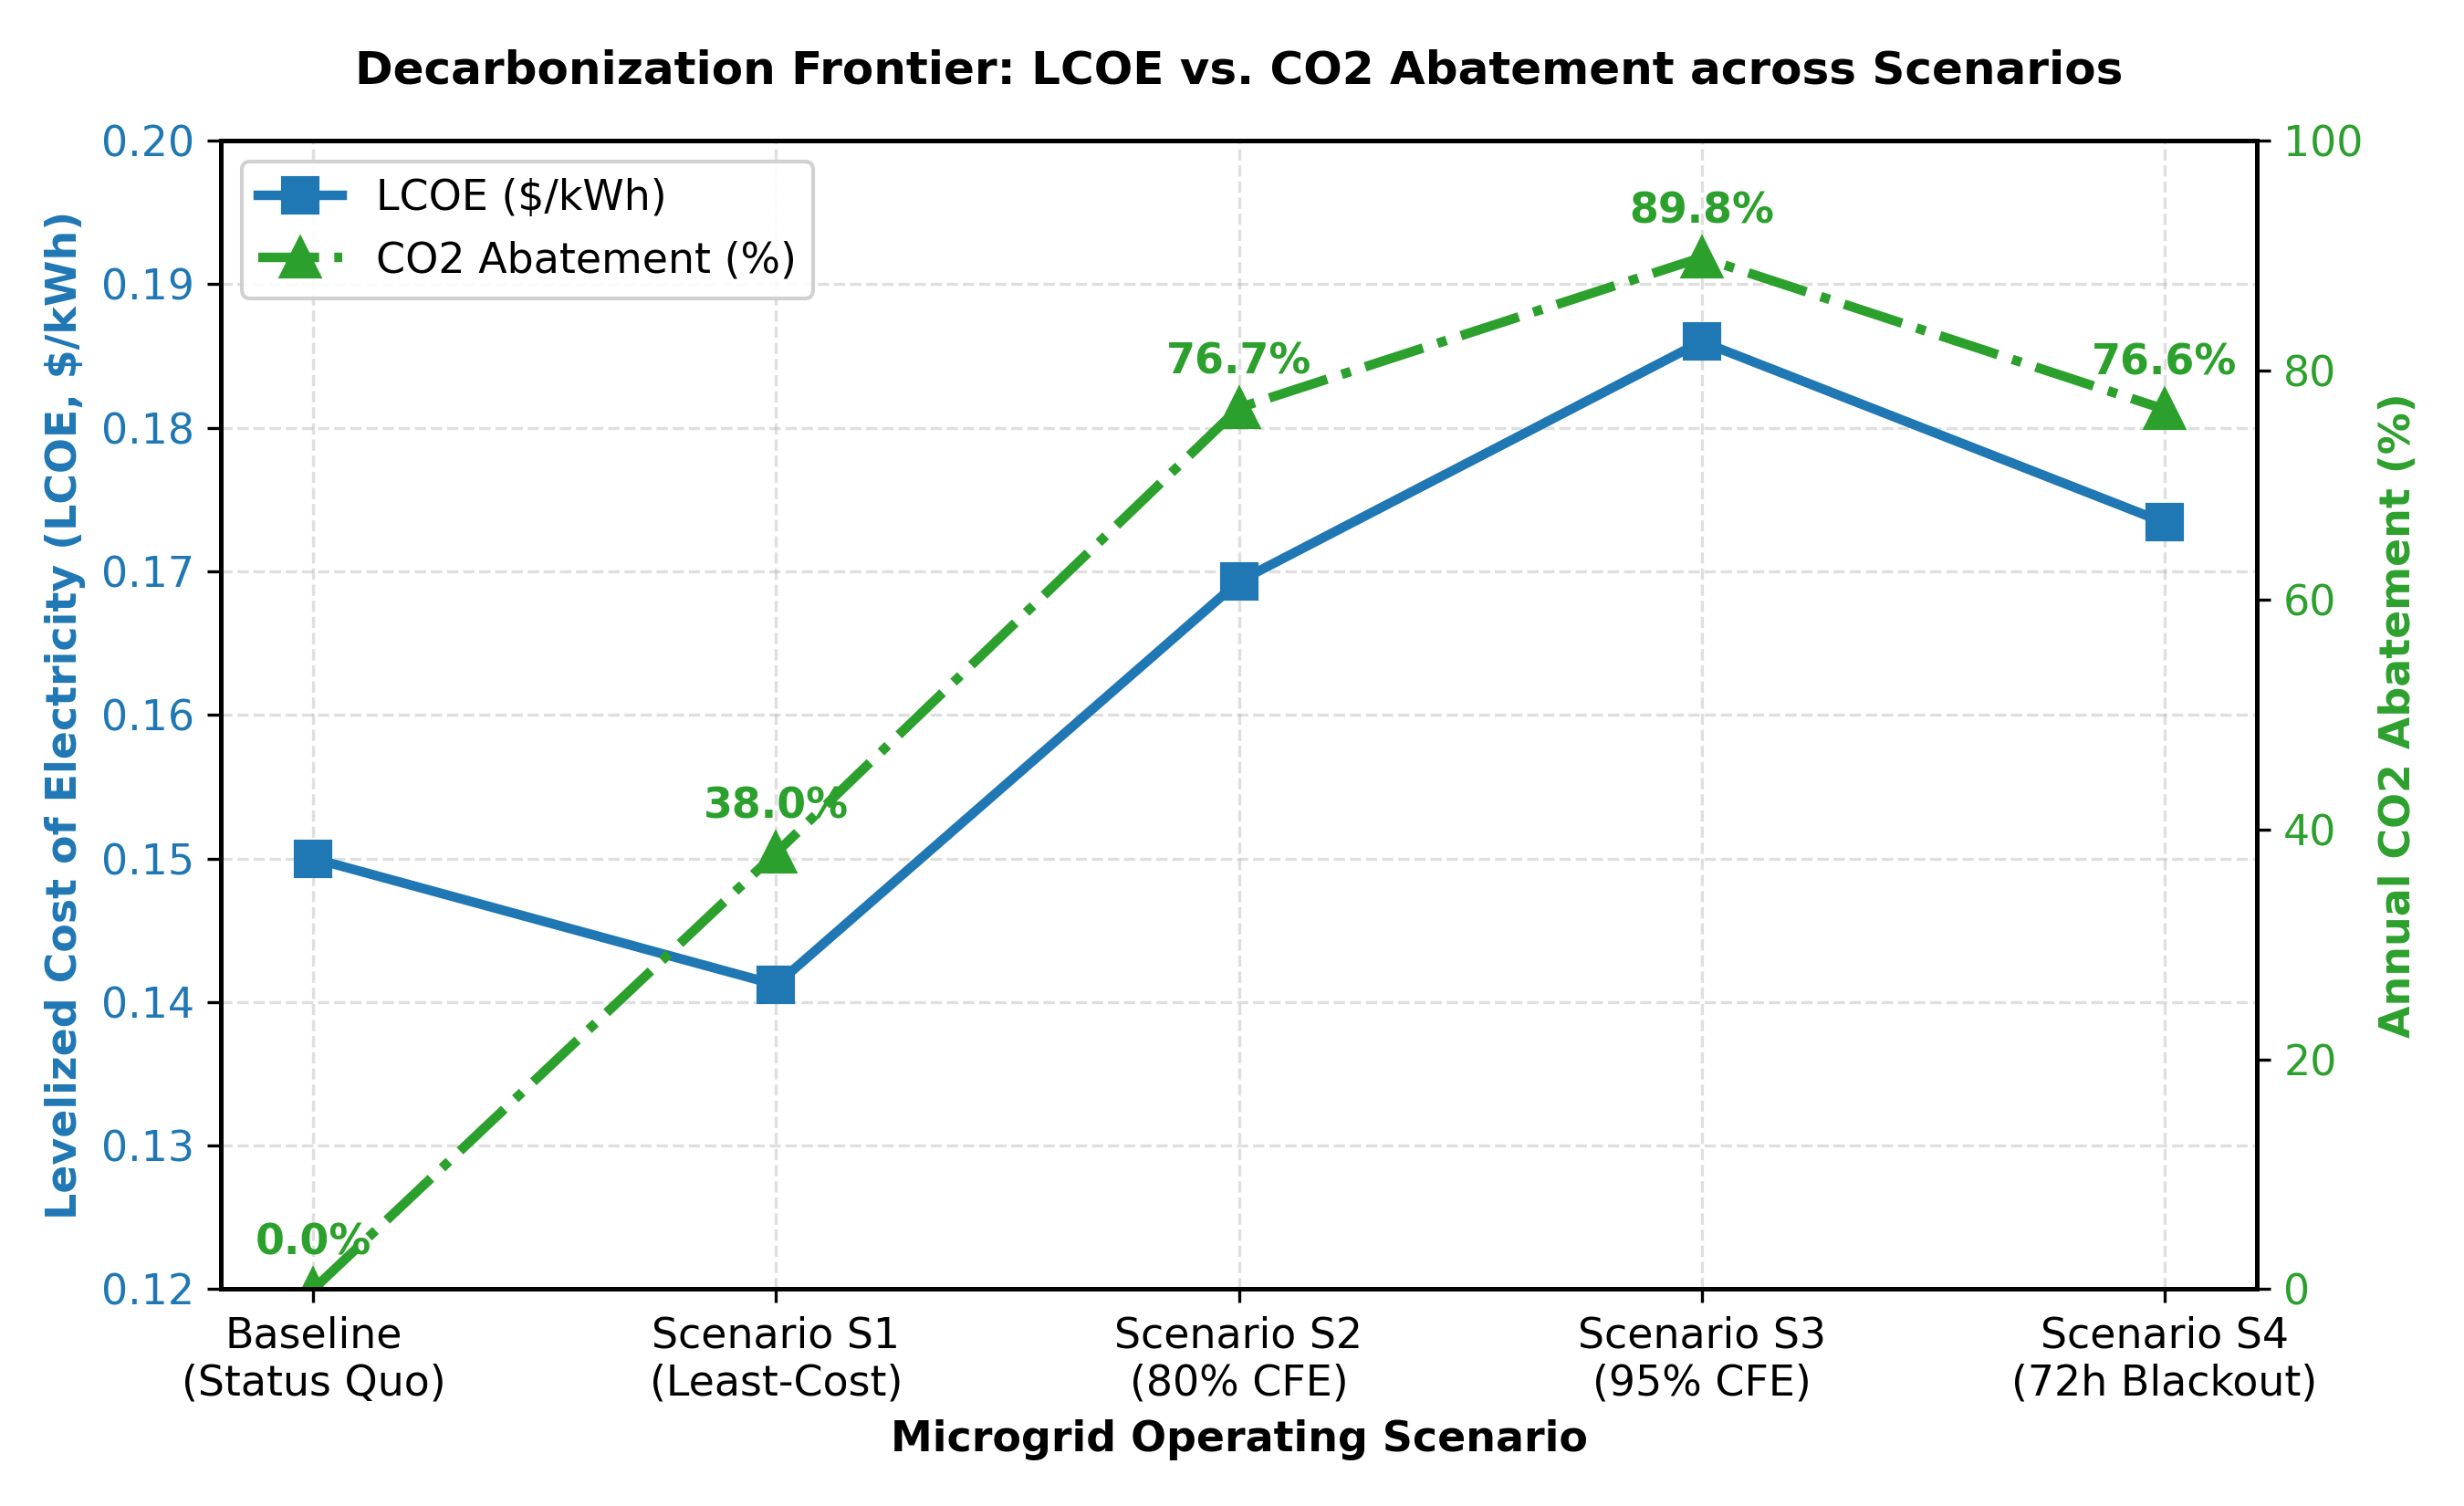
\includegraphics[width=0.92\textwidth]{Figures/Figure_2_Decarbonization_Pareto_Frontier.png}
\caption{Decarbonization Pareto Frontier: Levelized Cost of Energy (LCOE, \$/kWh) versus Annual CO$_2$ Emissions Abatement across scenarios S1, S2, S3, and S4. Dashed curves indicate the convex ``green premium'' zone beyond 80\% CFE matching.}
\label{fig:fig2}
\end{figure}

To capture the marginal 15\% of clean energy during cloudy wet-season conditions and consecutive low-solar days, BESS capacity must expand by 37.8\% (from 183.6~MWh to \textbf{253,105~kWh / 253.1~MWh}), while Solar PV expands to \textbf{113,845~kW (113.8~MW)}. This drives CapEx from \$142.85M to \$179.97M (+\$37.12M) and increases LCOE from \$0.1693/kWh to \$0.1860/kWh. While this configuration achieves an extraordinary 89.82\% carbon reduction (curbing emissions to 7,475~t/year), the marginal cost per ton of CO$_2$ abated rises exponentially, highlighting why hyperscalers may prefer hybrid bio-fuels or spatial workload migration to close the final 5--10\% clean energy gap.

Figure~\ref{fig:fig3} highlights the comparative physical asset allocations across all four architectures.

\begin{figure}[htbp]
\centering
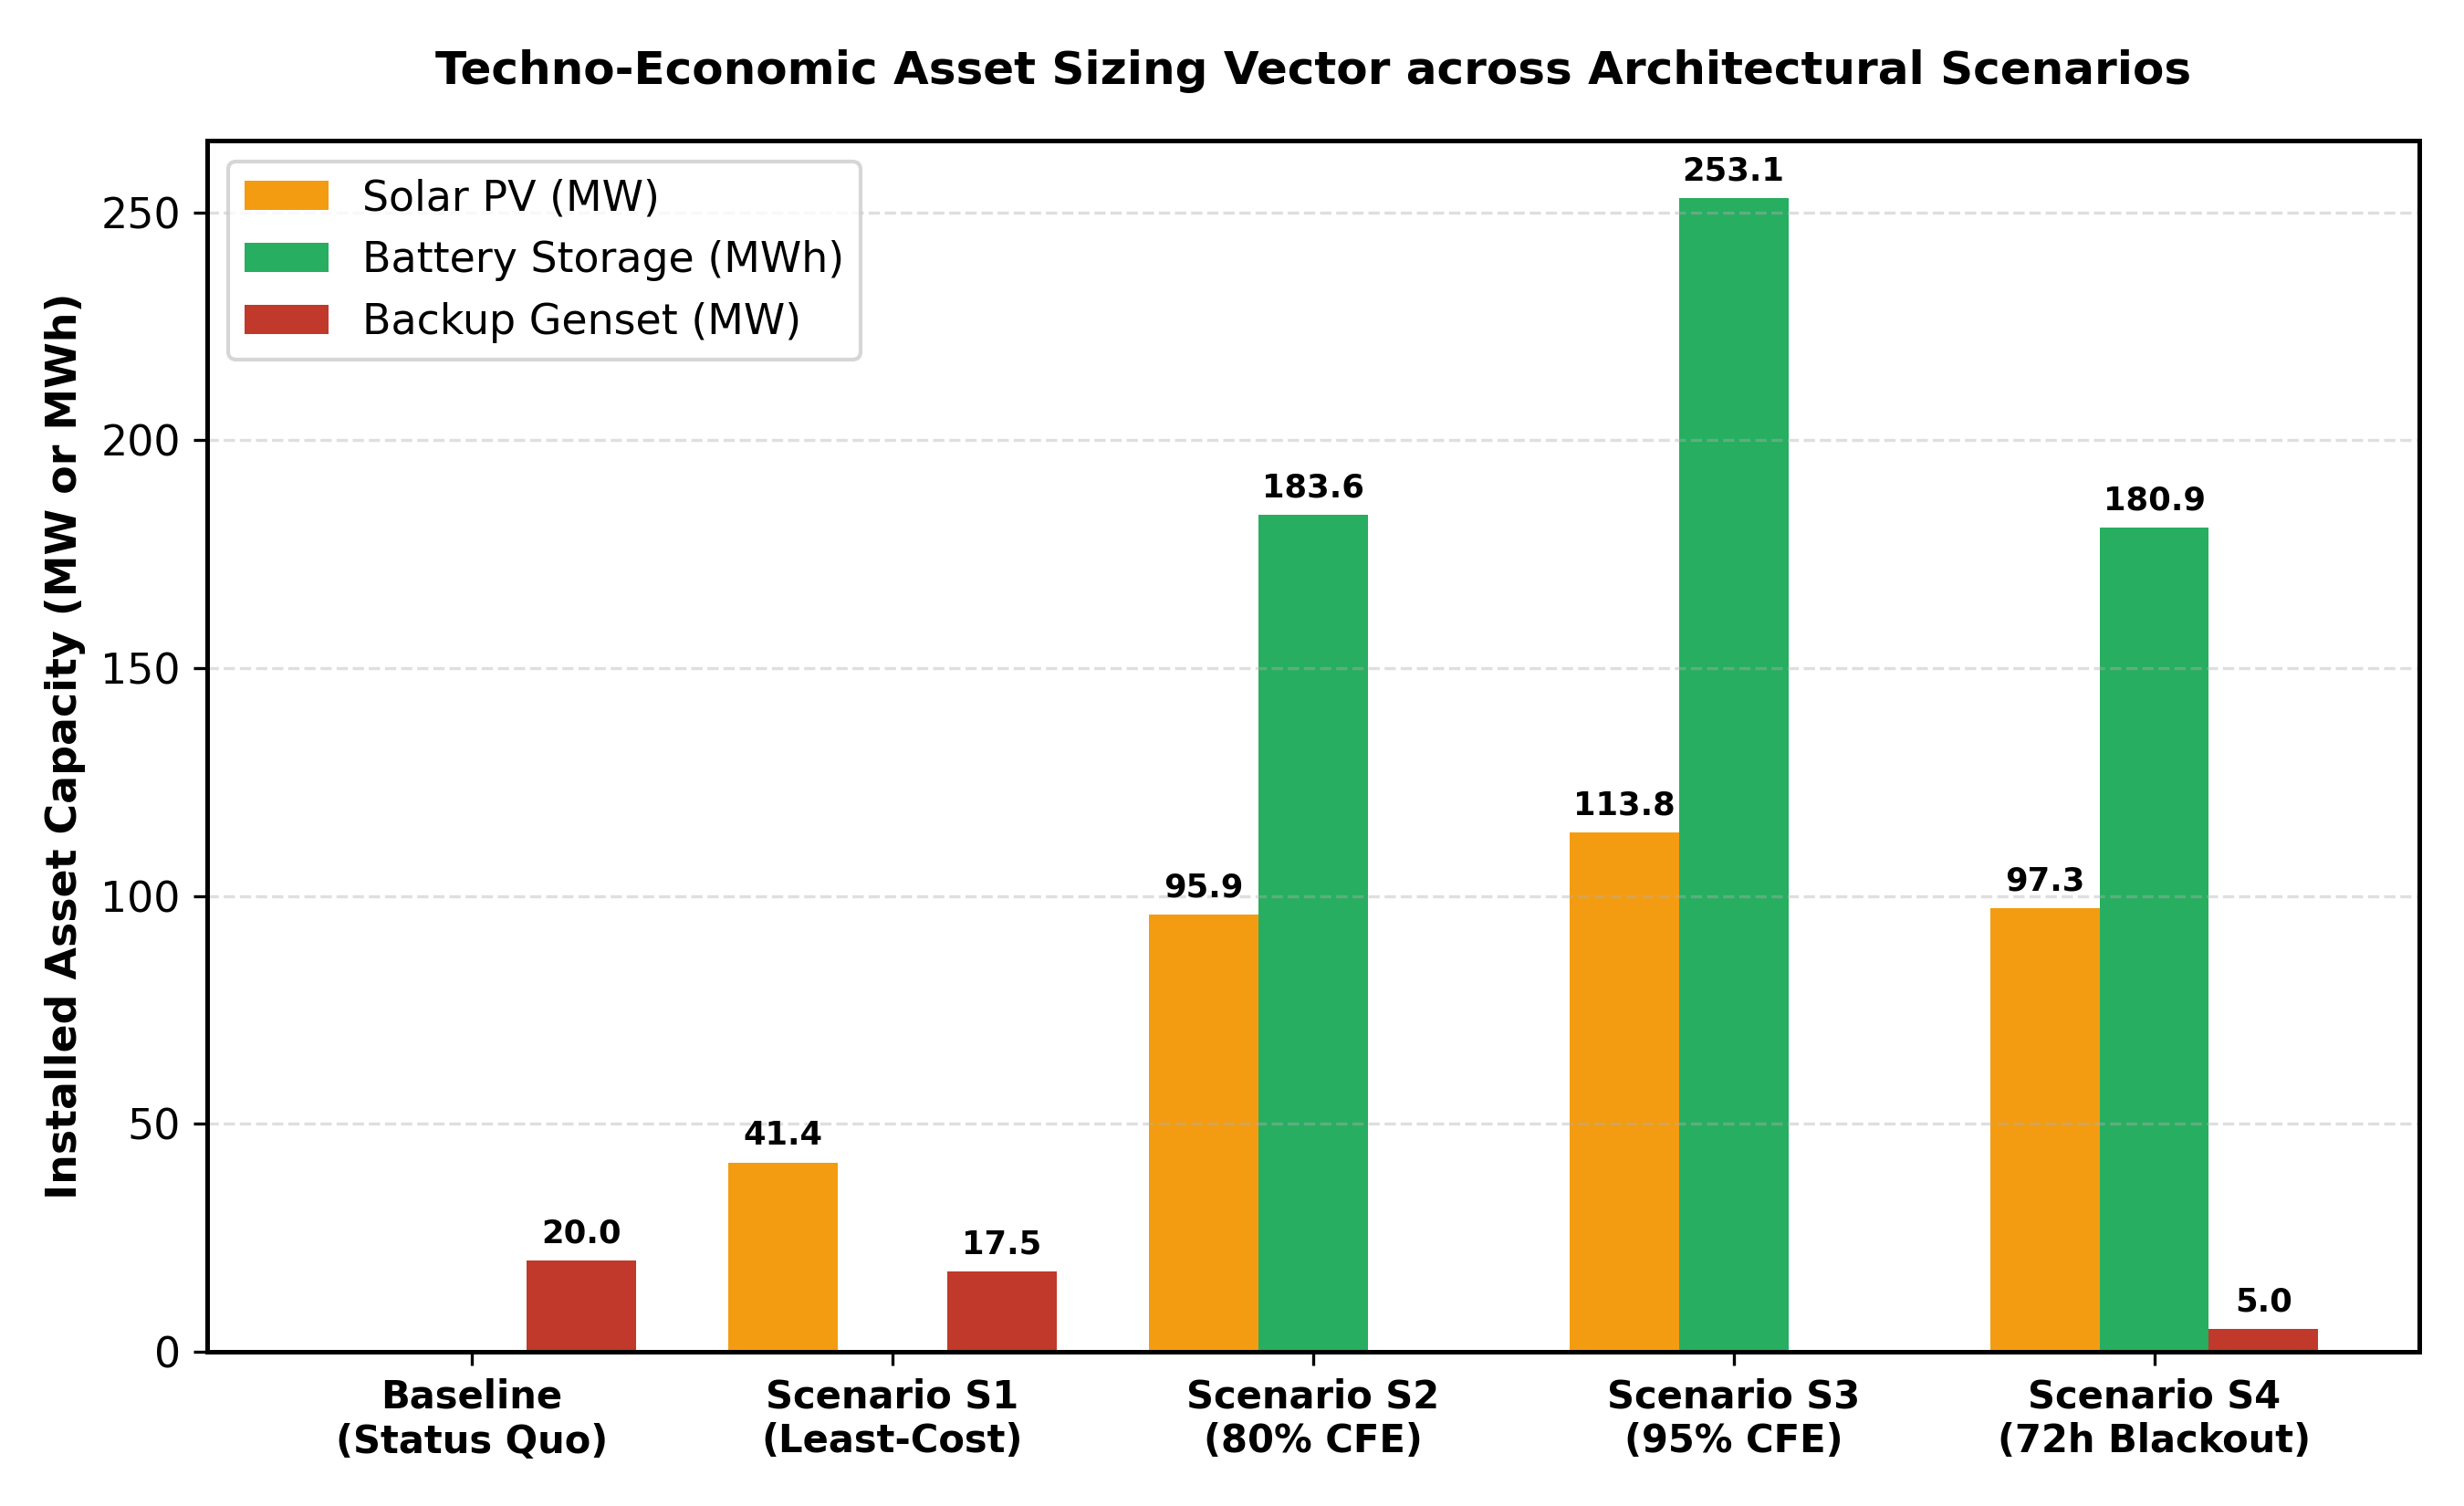
\includegraphics[width=0.95\textwidth]{Figures/Figure_3_Asset_Capacity_Sizing.png}
\caption{Asset capacity sizing comparison across scenarios. Demonstrates the transition from zero storage in S1 to massive storage deployment in S2 and S3, alongside the 71.4\% generator reduction achieved in S4.}
\label{fig:fig3}
\end{figure}

\subsection{Resiliency Optimization and Fleet Abatement under a 72-Hour Blackout (S4)}

In Scenario S4, the microgrid is subjected to a severe 72-hour continuous grid collapse during the rainy season. In standard data center engineering designs, surviving a multi-day blackout requires 100\% $N+1$ or $2N$ fossil generator redundancy ($20.0\text{ MW}$ to $25.0\text{ MW}$ of diesel engines), incurring severe fuel supply vulnerability and high capital expenditure.

Under the optimized solar-storage microgrid:
\begin{enumerate}
    \item \textbf{71.4\% Generator Fleet Reduction:} The backup generator fleet is reduced from 17.5~MW (in S1) down to just \textbf{5,000~kW (5.0~MW)}—a 71.4\% physical reduction.
    \item \textbf{Solar-Storage Cycling:} The 180.9~MWh BESS and 97.3~MW PV array supply the overwhelming majority of daytime and evening load. The two modular 2.5~MW diesel generators operate merely as peaking units to top up the battery bank during overcast afternoons.
    \item \textbf{Guaranteed Survivability:} The facility maintains a Loss of Load Probability ($\text{LOLP}$) of \textbf{0\%} throughout the 72-hour window.
\end{enumerate}

Figure~\ref{fig:fig4} displays the 20-year cumulative cash flow and capital payback trajectories.

\begin{figure}[htbp]
\centering
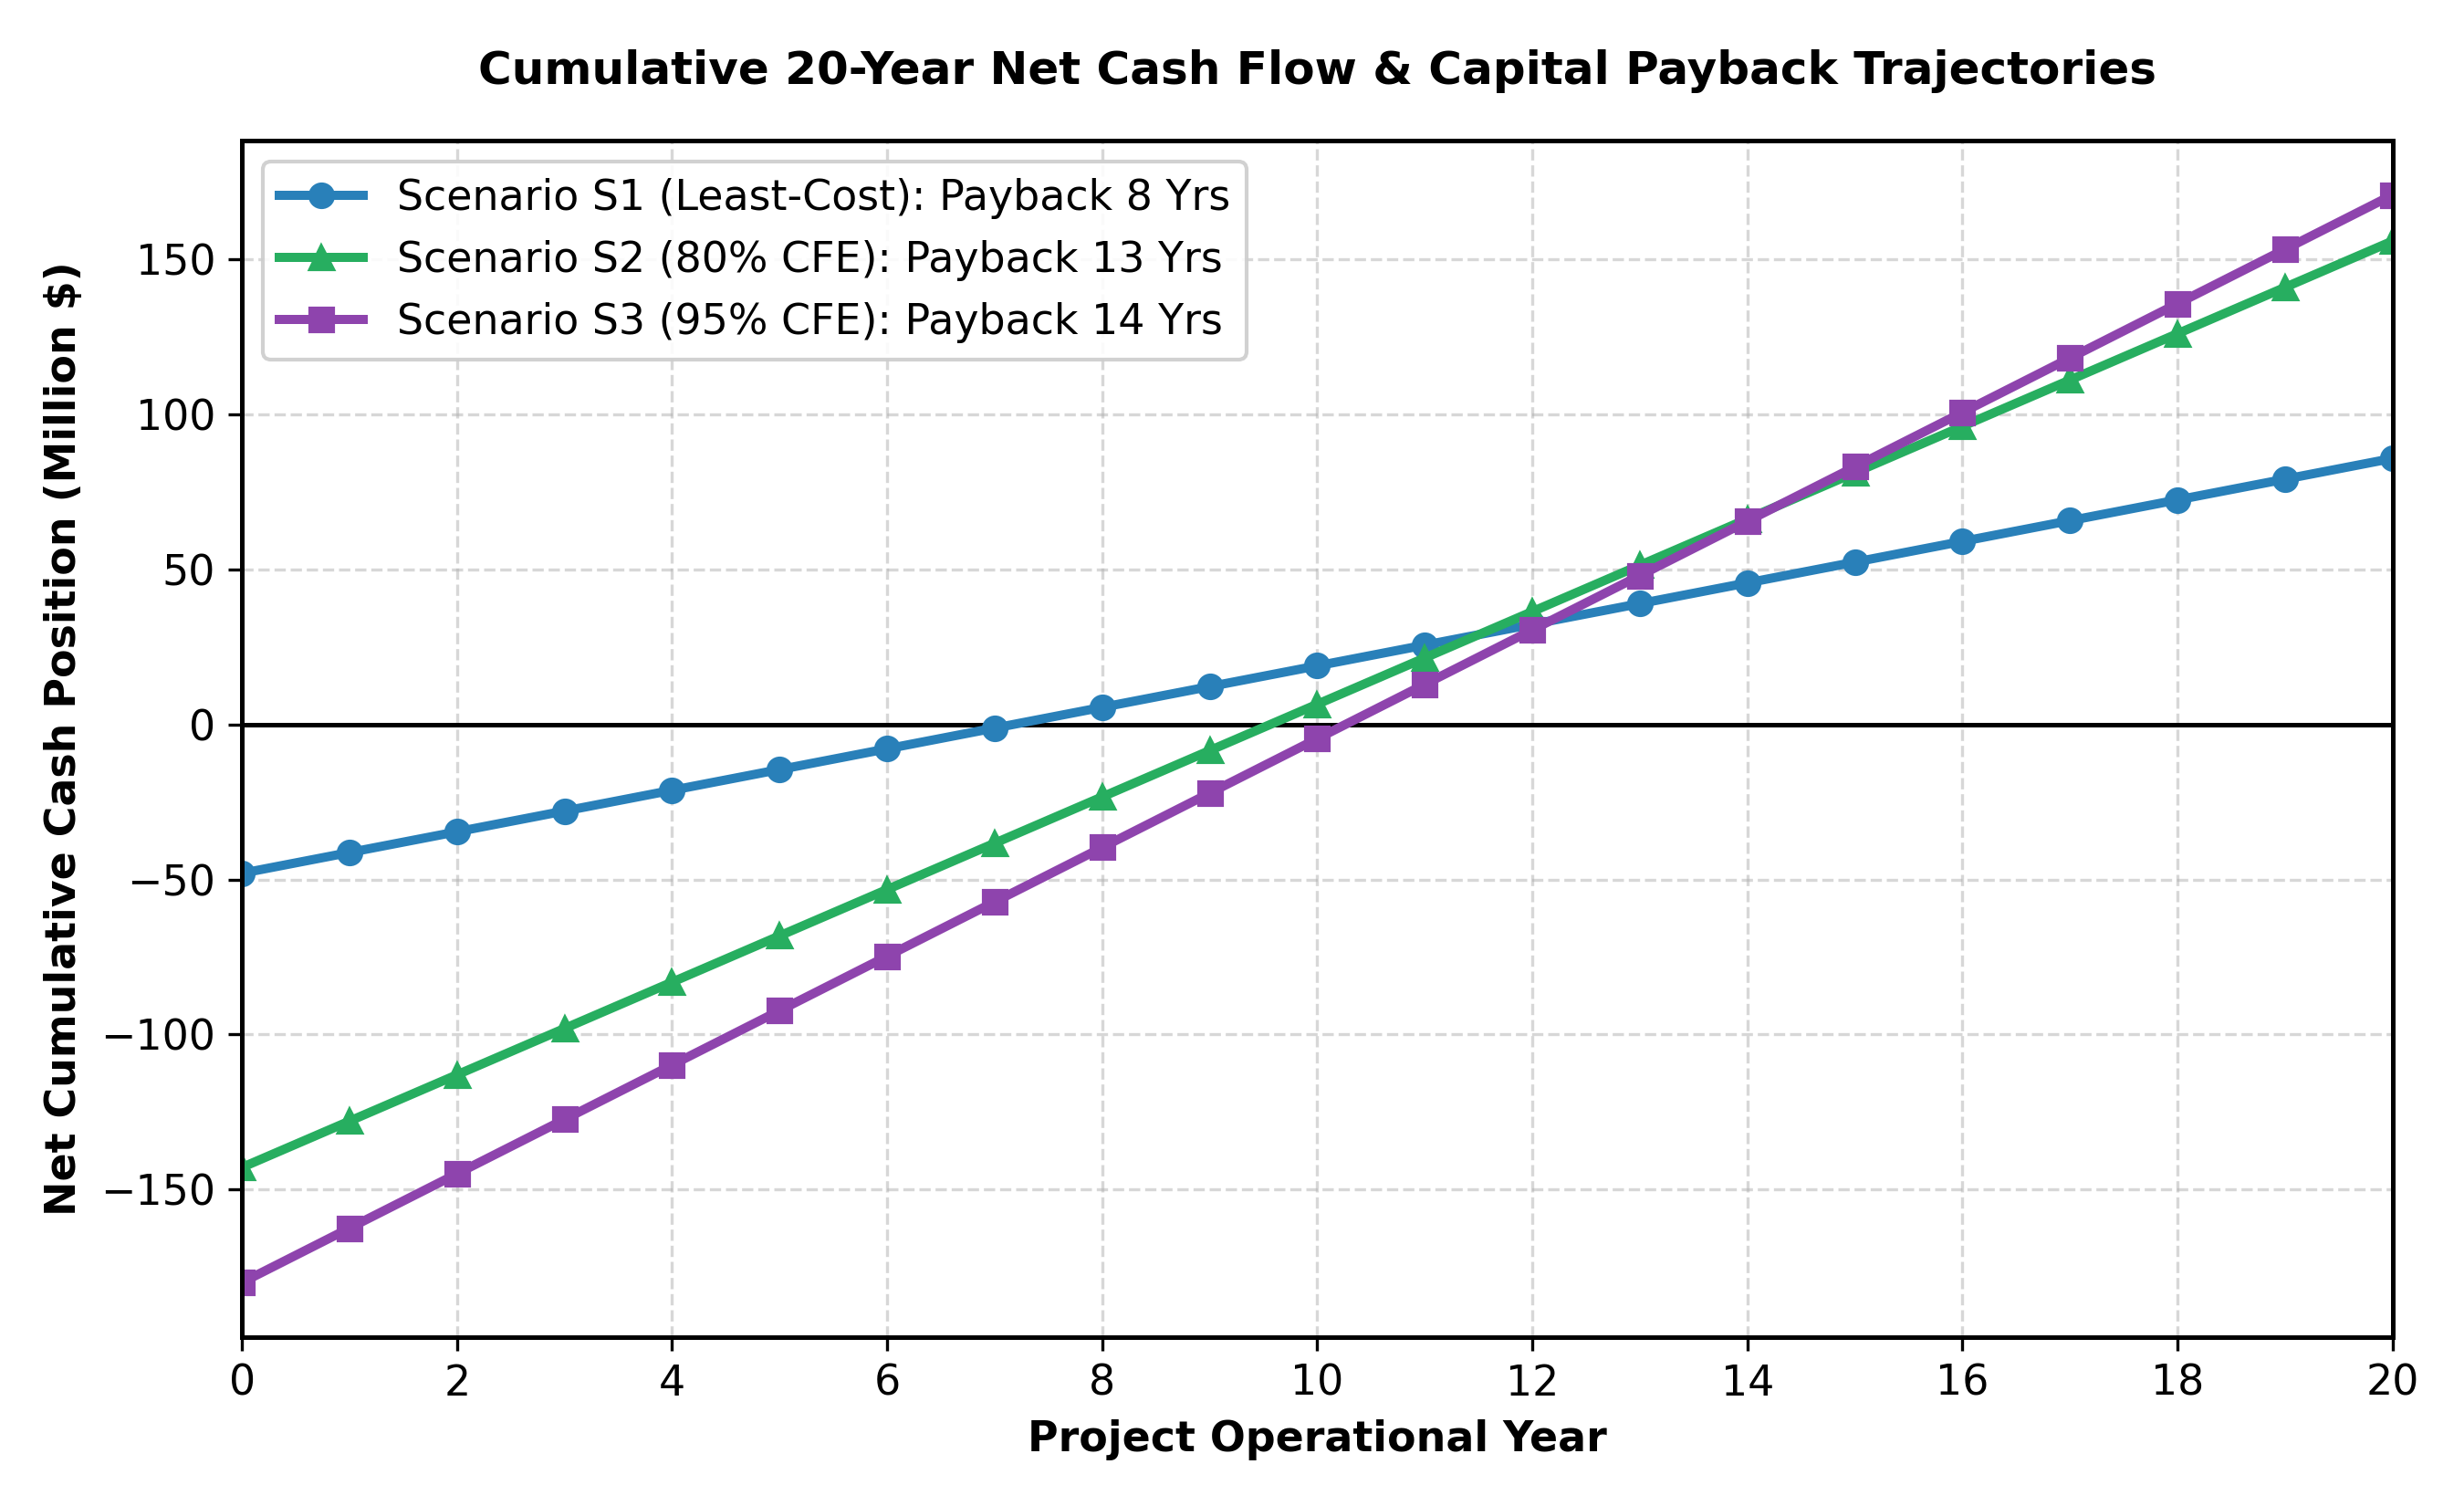
\includegraphics[width=0.92\textwidth]{Figures/Figure_4_Cumulative_Cash_Flow_Payback.png}
\caption{Cumulative net cash flows and capital payback trajectories over the 20-year project lifetime. While the baseline captive fossil system burns \$427M in cumulative operating costs, Scenario S2 breaks even at Year 13 and accumulates \$168M in net economic savings.}
\label{fig:fig4}
\end{figure}

\section{Policy and Industrial Implications}
\label{sec:policy}

\subsection{Regulatory Tariff and Wheeling Reforms (NERC)}
Under current Nigerian Electricity Regulatory Commission regulations, commercial microgrids are prohibited from injecting surplus power into the 330/132~kV transmission network. In Scenarios S2 and S3, mid-day solar curtailment reaches up to 15--22~MW during peak insolation hours when battery banks reach 90\% SoC. Establishing dynamic clean energy wheeling tariffs and localized peer-to-peer trading would enable hyperscalers to sell excess green power to adjacent industrial manufacturers in Ikeja, enhancing grid stability and reducing microgrid LCOE by an additional 12--18\%.

\subsection{Customs Duty Exemptions on Utility-Scale Storage}
BESS capital expenditure currently carries significant import tariffs and clearing surcharges at Nigerian ports. Because the 80\% CFE inflection point requires over 180~MWh of storage, federal fiscal policies exempting utility-scale lithium-ion battery containers from customs duties would accelerate data center decarbonization and protect national digital infrastructure against sovereign grid collapses.

\subsection{Escaping the Captive Diesel Trap}
As documented by the World Bank \cite{WorldBank2020}, Nigerian industrial consumers bear captive power costs exceeding \$0.40--\$0.46/kWh. By deploying an 80\% CFE solar-plus-storage microgrid, hyperscale AI campuses achieve an LCOE of \$0.1693/kWh—representing a cost reduction of over 58\% compared to self-generation diesel reliance, while delivering 99.999\% mission-critical availability.

\section{Conclusion}
\label{sec:concl}

This paper presented the first rigorous techno-economic and resiliency optimization of an AI data center microgrid operating within a weak-grid environment in Sub-Saharan Africa. By synthesizing an 8,760-hour computational load model coupling GPU cluster traces with ASHRAE TC 9.9 tropical chiller dynamics, we evaluated four distinct operational architectures in Lagos, Nigeria.

The primary conclusions are:
\begin{enumerate}
    \item \textbf{Economics Alone Excludes Storage:} Under least-cost optimization (S1), Solar PV (41.4~MW) without storage achieves an 8-year payback and \$0.1412/kWh LCOE, as nocturnal grid tariffs remain cheaper than amortized battery throughput.
    \item \textbf{80\% CFE Eliminates Captive Diesel:} Enforcing an 80\% clean energy mandate (S2) triggers 183.6~MWh of BESS and 95.9~MW of PV, completely ending captive diesel fuel combustion, reducing OpEx by 69.9\% (\$14.94M/yr saved), abating 76.7\% of carbon emissions, and breaking even within 13 years.
    \item \textbf{Resiliency and Generator Abatement:} The solar-storage microgrid guarantees 100\% survival across a 72-hour national grid collapse while slashing the required backup diesel generator fleet by 71.4\% (from 17.5~MW to 5.0~MW).
    \item \textbf{Escaping Fossil Lock-In:} Transitioning to solar-BESS unlocks levelized energy costs of \$0.1693/kWh, delivering dramatic financial savings over the \$0.40--\$0.46/kWh captive diesel baseline documented across Nigerian industry.
\end{enumerate}

These empirical findings provide the first actionable engineering and policy blueprint for powering the next generation of artificial intelligence across the Global South.

\section*{Declaration of Competing Interest}
The authors declare that they have no known competing financial interests or personal relationships that could have appeared to influence the work reported in this paper.

\section*{Data Availability Statement}
The synthesized 8,760-hour AI workload profile, tropical PUE curves, and complete Xendee simulation optimization output datasets are openly accessible in the project repository.

\bibliographystyle{elsarticle-num}
\bibliography{references}

\end{document}
